\chapter{整机调试问题记录}
\label{cha:Debug}

\section{待机状态下电机发热}

2020年4月12日下午三点多在调试小车运动的时候,使用了如下代码在PCBv2上进行了测试:

\inputminted[mathescape, linenos, breaklines]{c}{Code/Stepper-3-Movement/Stepper-3-Movement.ino}

连上电池、烧写程序、等待五秒后两电机经过加减速过程反向转动10000 Step后停止,推动小车向前运动一段距离。

但是在电机停止后我没有像往常一样拔下锂电池,大约十分钟,我闻到了金属加热后表面涂层的焦糊气味(有点像电弧焊的气味),寻找来源的过程中感受到了小车的热辐射,第一反应就是把锂电池拔下来,感受到锂电并没有发热松了一口气,大致判定是电机发热,我做了一个错误决定,用手指伸到了电机外壳上验证是不是电机在发热,感受到电机温度应该在200-300摄氏度之间,手指被烫伤。

怀疑是Speed=0时AccelStepper库依然在向DRV8825发送比较低频的PWM信号,使得有大电流持续通过电机绕组。

目前3D打印的小车底盘已经部分融化变形(熔点150摄氏度),如图~\ref{fig:DebugHeat}。

% 如果我碰巧离开工位,温度会继续上升,可能会引发火灾。

\begin{figure}[htbp]
    \centering
    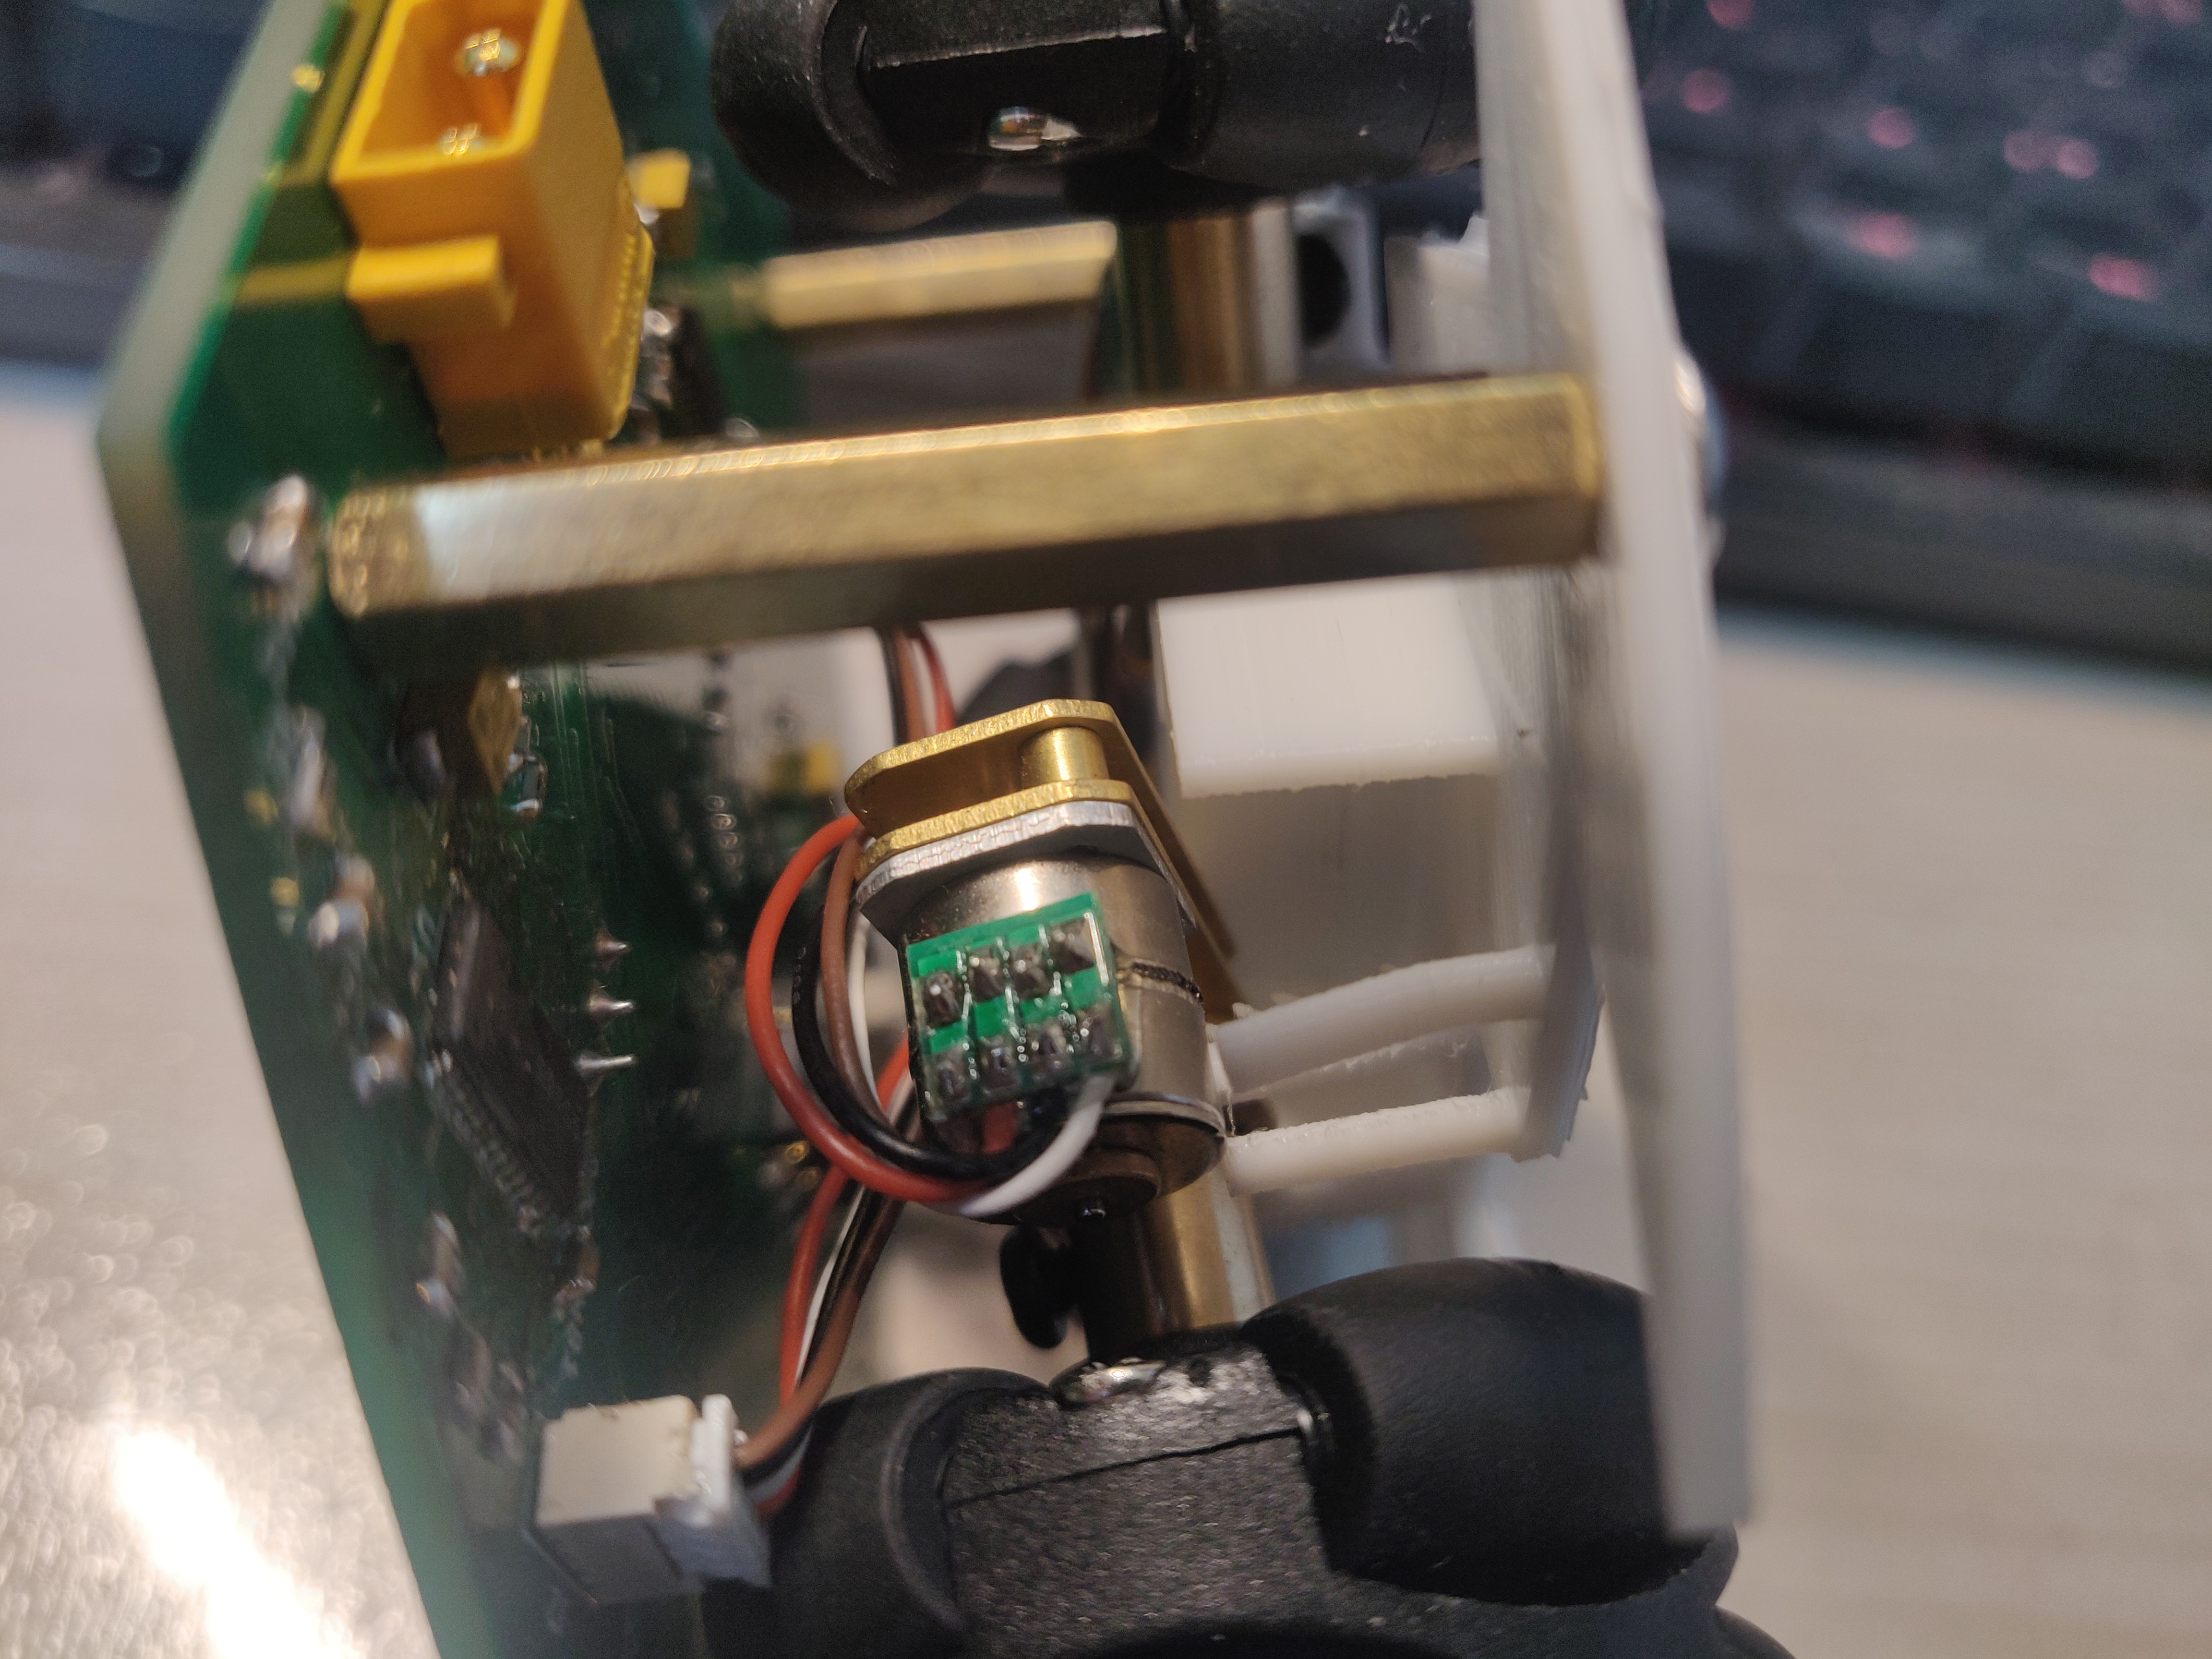
\includegraphics[width=\columnwidth]{DebugHeat.jpg}
    \caption{融化变形的PLA电机固定}
    \label{fig:DebugHeat}
\end{figure}

得到以下经验教训:

\begin{enumerate}
    \item 将来调试完成后立即断开锂电的连接,同时调试时间也控制在一分钟以内以减少发热量。
    \item 购买二氧化碳灭火器放在工位旁以防万一。
    \item 感受到热浪和焦糊味要保持清醒头脑,不要贸然触碰可能的发热点。
\end{enumerate}


\section{时钟问题}

时钟周期比我代码设定的长了16倍,原因未知。

测试代码如下:

\inputminted[mathescape, linenos, breaklines]{c}{Code/PWM-Test/PWM-Test.ino}

测得波形数据如图~\ref{fig:DebugClock}。

\begin{figure}[htbp]
    \centering
    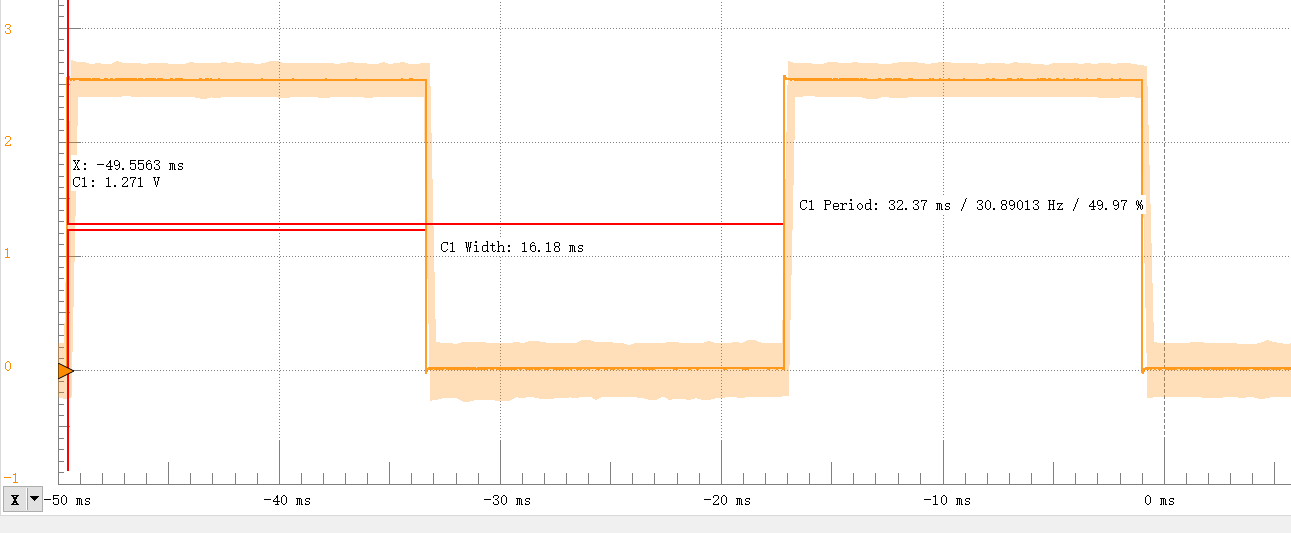
\includegraphics[width=\columnwidth]{DebugClock.png}
    \caption{实测时钟周期}
    \label{fig:DebugClock}
\end{figure}
